\section{Radix Sort}
\label{sec:radix sort}

This this section will present a parrallized algorithm of the radix sort benchmarked with a serial sort implementation from the C++ library.
The implementation of the Radix Sort algorithm can be found in \cref{ap:radix sort}.

Radix Sort is a bit-wise comparison algorithm that iteratively, in the length of the bits of the integer, looks at the LSB and sorts the values accordingly.\cite{udacity}

In order to parralelize the sorting of the LSB in the radix sort we used the compact(\cref{sec:compact}).  
Thus, the radix sort is performed with multiple compact operations, because we move elements according to some predicate.
We aim to outline a single iteration of radix sort in this section.

% iteratively do for each bit

\paragraph{Compute Predicates}
The first step is to find the elements that obey the predicate.
For radix sort we look at the LSB of every bit of the integers.
The predicate is as presented in \cref{lst:predicate radix}.

\begin{lstlisting}[caption={predicate to calculate}, label={lst:predicate radix}]
d_predicate[mid] = (int)(((d_val_src[mid] & (1 << i)) >> i) == 0)
\end{lstlisting}

The \ttt{d\_predicate} will contain 0s and 1s.
If the LSB is 0, it will contain a 1 for that element.
The elements in \ttt{d\_val\_src} are traversed and labelled accordingly.

For each iteration of the outer loop, we count the \ttt{i} variable up.
This way we can left shift the integer 1 by \ttt{i} positions to move to the next LSB in the row.
When perform the bitwise-and, and shift it back to see if it is equal to 0.

Furthermore, we save a new predicate array, \ttt{d\_predicate\_toggle}, where we save the toggled version of the original \ttt{d\_predicate}.
This array gives us the elements that did not obey the predicate.
We do this, because we must maintain the order of the elements in the output array.

\subsection*{Compute Scatter Addresses}

To be able to move the elements to their new positions according to the predicate, we can perform an exclusive sum scan of the predicate array.
This gives the addresses to which the elements must be scattered.
We performed an exclusive sum scan by first invoking a Hillis and Steele inclusive sum scan and then shifting the resulting array to obtain an exclusive sum scan.

For the toggled predicate array we must include an offset that is equal to the amount of elements, that did obey the initial predicate.
Thus, we must add an offset to the scatter addresses computed from the toggled predicate array.
We do this by performing a reduce operation on the original predicate array, which gives us the amount of elements that had LSB to 0.
We then do a mapping operation to add the offset to each element of the scatter address array.

The elements should then be scattered to the new addresses according to the LSB.
This is briefly illustrated in \cref{fig:radix sort example}.
This method should then be continued for each bit.
We continue to the next bit by incrementing the variable \ttt{i}, and perform the bitwise-and as illustrated in \cref{lst:predicate radix}.

\begin{figure}[htb]
  \centering
  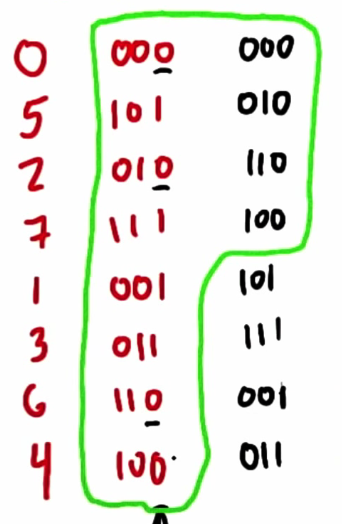
\includegraphics[height=4cm]{images/radix-sort-example.png}
  \caption{Example of how each digit is moved according to LSB}
  \label{fig:radix sort example}
\end{figure}


%\subsection*{Iterating through each Bit}
%
%\begin{lstlisting}
%for ( unsigned int i = 0; i < (BITS_PER_BYTE * sizeof( unsigned int)); i++) {
%  // predicate is that LSB is 0
%  predicate_kernel<<<GRID_SIZE, BLOCK_SIZE>>>(d_predicate, d_val_src, NUM_ELEMS, i);
%  // calculate scatter addresses from predicates
%  exclusive_sum_scan(d_sum_scan_0, d_predicate, d_predicate_tmp, d_sum_scan, ARRAY_BYTES, NUM_ELEMS, GRID_SIZE, BLOCK_SIZE);
%  // copy contents of predicate , so we do not change its content
%  checkCudaErrors(cudaMemcpy(d_predicate_tmp, d_predicate, ARRAY_BYTES, cudaMemcpyDeviceToDevice));
%  // calculate how many elements had predicate equal to 1
%  reduce_wrapper(d_reduce, d_predicate_tmp, NUM_ELEMS, BLOCK_SIZE);
%  // toggle predicate values , so we can compute scatter addresses for toggled predicates
%  toggle_predicate_kernel<<<GRID_SIZE, BLOCK_SIZE>>>(d_predicate_toggle ,d_predicate, NUM_ELEMS);
%  // so we now have addresses for elements where LSB is equal to 1
%  exclusive_sum_scan(d_sum_scan_1, d_predicate_toggle, d_predicate_tmp, d_sum_scan, ARRAY_BYTES, NUM_ELEMS, GRID_SIZE, BLOCK_SIZE);
%  // shift scatter addresses according to amount of elements that had LSB equal to 0
%  add_splitter_map_kernel<<<GRID_SIZE, BLOCK_SIZE>>>(d_sum_scan_1, d_reduce, NUM_ELEMS);
%  // move elements accordingly
%  map_kernel<<<GRID_SIZE, BLOCK_SIZE>>>(d_map, d_val_src, d_predicate, d_sum_scan_0, d_sum_scan_1, NUM_ELEMS);
%  // swap pointers , instead of moving elements
%  std::swap(d_val_src, d_map);
%}
%\end{lstlisting}
